\documentclass[12pt]{report}
\usepackage[utf8]{inputenc}
\usepackage{a4}
\usepackage[none]{hyphenat} %hyphenation
\sloppy
\usepackage{parskip} %no indentation after paragraphs
\usepackage{afterpage} %for using \afterpage{\clearpage} (don't push images to the end of a chapter)
\usepackage{makeidx}
\usepackage[numbers]{natbib}
\usepackage{picins} %provides precise control over the placement of inline graphics
\usepackage{setspace}
\usepackage{titlesec}
\usepackage{dsfont} %math symbols
\usepackage{tabularx}
\usepackage{floatflt} %float text around figures and tables
\usepackage{enumitem} %resume counting from previous enumerate block
\usepackage{amsmath,amssymb}
\usepackage[format=default,font=footnotesize,labelfont=bf]{caption}
\usepackage{listings} %for listing source code
\usepackage{color}
\usepackage{float} % for [H] after floats
\usepackage{url}
\usepackage{graphicx} 
\usepackage{todonotes}
\usepackage[automake]{glossaries}
\newglossary[slg]{symbolslist}{syi}{syg}{Symbols}
\makeglossaries
\newacronym{SA}{SA}{Sample Abbreviation}
 % all abbreviations
\newglossaryentry{symb:N}{sort={3},
name={$\mathbb N$},
first={first $\mathbb N$},
text={additional $\mathbb N$},
description={Set of natural numbers},
type=symbolslist} % all symbols
\glsaddall[types=\acronymtype]
\usepackage{listings}
\usepackage{color}
\definecolor{gray}{rgb}{0.4,0.4,0.4}
\definecolor{darkblue}{rgb}{0.0,0.0,0.6}
\definecolor{cyan}{rgb}{0.0,0.6,0.6}
\definecolor{dkgreen}{rgb}{0,0.6,0}
\definecolor{gray}{rgb}{0.5,0.5,0.5}
\definecolor{mauve}{rgb}{0.58,0,0.82}
\usepackage[autostyle]{csquotes}
\usepackage{subcaption}
\usepackage[ruled,lined,linesnumbered, noend]{algorithm2e}
\usepackage{algorithmicx}
\usepackage{algpseudocode}
\usepackage[]{algorithm2e}
\usepackage{multirow}
\usepackage{rotating}
\usepackage[toc,page]{appendix}
\usepackage{CJKutf8}
\usepackage{longtable}

\lstdefinestyle{myScalastyle}{
  frame=tb,
  language=scala,
  aboveskip=3mm,
  belowskip=3mm,
  showstringspaces=false,
  columns=flexible,
  basicstyle={\small\ttfamily},
  numbers=none,
  numberstyle=\tiny\color{gray},
  keywordstyle=\color{blue},
  commentstyle=\color{dkgreen},
  stringstyle=\color{mauve},
  frame=single,
  breaklines=true,
  breakatwhitespace=true,
  tabsize=3,
}

\setlength{\extrarowheight}{10pt}

\lstset{
	basicstyle=\ttfamily,
	columns=fullflexible,
	showstringspaces=false,
	commentstyle=\color{gray}\upshape
}

\titleformat{\paragraph}[hang]{\normalfont\bfseries}{\theparagraph}{.5em}{}

\makeindex
\frenchspacing
\sloppy
\pagestyle{headings}
\textwidth16cm
\textheight22cm
\topmargin0cm
\oddsidemargin0cm
\evensidemargin0cm

\newcommand\tab[1][1cm]{\hspace*{#1}}

\newcommand{\bildklein}[3]{  
	\begin{figure}[hp]
	\begin{center}
	\includegraphics[width=0.5\textwidth]{#1}
	\end{center}
	\caption[#2]{#3}
	\end{figure}
}	
\newcommand{\bildgross}[3]{  
	\begin{figure}[hp]
	\begin{center}
	\includegraphics[width=0.95\textwidth]{#1}
	\end{center}
	\caption[#2]{#3}
	\end{figure}
}

% This is tumlogo.tex
%
% Neues TUM-Logo in TeX
%   by G. Teege, 19.10.89
% Benutzung:
%   Am Anfang des Dokuments (TeX oder LaTeX):
%     \input tumlogo
%   Dann beliebig oft:
%     \TUM{<breite>}
%   bzw.
%     \oTUM{<breite>}
%   \TUM setzt das Logo mit der Breite <breite> und der entsprechenden Hoehe.
%   <breite> muss eine <dimen> sein. \oTUM erzeugt eine "outline"-Version
%   des Logos, d.h. weiss mit schwarzem Rand. Bei \TUM ist es ganz schwarz.
%   \oTUM entspricht damit der offiziellen Version des Logos.
%   Das Logo kann wie ein einzelnes Zeichen verwendet werden.
%   Beispiel:
%     Dies ist das TUM-Logo: \oTUM{1cm}.
%
\def\TUM#1{%
\dimen1=#1\dimen1=.1143\dimen1%
\dimen2=#1\dimen2=.419\dimen2%
\dimen3=#1\dimen3=.0857\dimen3%
\dimen4=\dimen1\advance\dimen4 by\dimen2%
\setbox0=\vbox{\hrule width\dimen3 height\dimen1 depth0pt\vskip\dimen2}%
\setbox1=\vbox{\hrule width\dimen1 height\dimen4 depth0pt}%
\setbox2=\vbox{\hrule width\dimen3 height\dimen1 depth0pt}%
\setbox3=\hbox{\copy0\copy1\copy0\copy1\box2\copy1\copy0\copy1\box0\box1}%
\leavevmode\vbox{\box3}}
%
\def\oTUM#1{%
\dimen1=#1\dimen1=.1143\dimen1%
\dimen2=#1\dimen2=.419\dimen2%
\dimen3=#1\dimen3=.0857\dimen3%
\dimen0=#1\dimen0=.018\dimen0%
\dimen4=\dimen1\advance\dimen4 by-\dimen0%
\setbox1=\vbox{\hrule width\dimen0 height\dimen4 depth0pt}%
\advance\dimen4 by\dimen2%
\setbox8=\vbox{\hrule width\dimen0 height\dimen4 depth0pt}%
\advance\dimen4 by-\dimen2\advance\dimen4 by-\dimen0%
\setbox4=\vbox{\hrule width\dimen4 height\dimen0 depth0pt}%
\advance\dimen4 by\dimen1\advance\dimen4 by\dimen3%
\setbox6=\vbox{\hrule width\dimen4 height\dimen0 depth0pt}%
\advance\dimen4 by\dimen3\advance\dimen4 by\dimen0%
\setbox9=\vbox{\hrule width\dimen4 height\dimen0 depth0pt}%
\advance\dimen4 by\dimen1%
\setbox7=\vbox{\hrule width\dimen4 height\dimen0 depth0pt}%
\dimen4=\dimen3%
\setbox5=\vbox{\hrule width\dimen4 height\dimen0 depth0pt}%
\advance\dimen4 by-\dimen0%
\setbox2=\vbox{\hrule width\dimen4 height\dimen0 depth0pt}%
\dimen4=\dimen2\advance\dimen4 by\dimen0%
\setbox3=\vbox{\hrule width\dimen0 height\dimen4 depth0pt}%
\setbox0=\vbox{\hbox{\box9\lower\dimen2\copy3\lower\dimen2\copy5%
\lower\dimen2\copy3\box7}\kern-\dimen2\nointerlineskip%
\hbox{\raise\dimen2\box1\raise\dimen2\box2\copy3\copy4\copy3%
\raise\dimen2\copy5\copy3\box6\copy3\raise\dimen2\copy5\copy3\copy4\copy3%
\raise\dimen2\box5\box3\box4\box8}}%
\leavevmode\box0}
% End of tumlogo.tex



\begin{document}

\hoffset=5mm
\thispagestyle{empty}
\begin{center}
	\bigskip \bigskip \bigskip 
	\oTUM{6.0cm} \\
	\vspace*{0.8cm}
	{\huge \bf Technische Universität} \\
	\bigskip
	{\huge \bf München} \\
	\bigskip \bigskip \bigskip
	{\huge \bf Fakultät für Information Systems} \\
	\bigskip \bigskip \bigskip
	{\Large \bf Master's Thesis in Informatik} \\
	\bigskip \bigskip \bigskip \bigskip \bigskip
	{\Large  Bitcoin-like Blockchain Simulation System} \\        
	\bigskip \bigskip \bigskip \bigskip
	{\Large Fabian Schüssler} \\    
	\bigskip
	\begin{figure}[ht]
	\centering 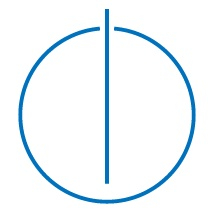
\includegraphics[width=0.2\linewidth]{figures/infologo.jpg}
	\end{figure}
	\bigskip 
\end{center}
\vfill

\newpage
\hoffset=5mm
\thispagestyle{empty}
\begin{center}
	\bigskip \bigskip \bigskip 
	\oTUM{6.0cm} \\
	\vspace*{0.8cm}
	{\huge \bf Technische Universität} \\
	\bigskip
	{\huge \bf München} \\
	\bigskip \bigskip \bigskip
	{\huge \bf Fakultät für Informatik} \\
	\bigskip \bigskip \bigskip
	{\Large \bf Master's Thesis in Information Systems} \\
	\bigskip \bigskip \bigskip \bigskip \bigskip
	{\Large Bitcoin-like Blockchain Simulation System} \\
	\bigskip \bigskip \bigskip
	{\Large Bitcoin-ähnliches Blockchain Simulationssystem} \\
	\bigskip
\end{center}
\vfill
\begin{tabular}{ll}
{\Large \bf Author:} & {\Large Fabian Schüssler} \\\\
{\Large \bf Supervisor:} & {\Large Prof. Dr. Hans-Arno Jacobsen} \\\\
{\Large \bf Advisor:} & {\Large Pezhman Nasirifard} \\\\
{\Large \bf Submission:} & {\Large xx.xx.20xx}
\end{tabular}

\newpage	
\thispagestyle{empty}
\hoffset=0mm
\vspace*{\fill}
\noindent I confirm that this master's thesis is my own work and I have documented all sources and material used.\\\\
München, xx.xx.20xx\\\\\\\\\\\\
\noindent \textit{(Fabian Schüssler)}

\newpage
\thispagestyle{empty}
\null

\newpage
\thispagestyle{empty}
\hoffset=0mm
\section*{Abstract}	
\begin{spacing}{1.2}
Despite the recent \$600 billion crash and the high volatility of the whole cryptocurrency market, interest in development and research on blockchains is growing. Reaching the scalability of more traditional payment processors like PayPal or VISA is still a hard problem for decentralized peer-to-peer networks like bitcoin. Heated debates about scalability solutions led to the creation of hardforks like bitcoin cash. For users to better understand the impact of changes to the bitcoin protocol on scalability and security and to find optimal solutions, we propose Bitcoin-like Blockchain Simulation System (BBSS). BBSS is a configurable bitcoin-like blockchain simulator. Its focus is on the visualisation of the simulation results to make every blockchain detail easy to understand. With block size limits, transaction fees, Segregated Witness and other features the Scalability Problem can be analysed. The optional attacks double-spending and transaction spam allow examination of security properties. The design and architecture allow large-scale simulations in a comparatively short amount of time.
\end{spacing}
 
\newpage
\thispagestyle{empty}
\hoffset=0mm
\section*{Inhaltsangabe}
\begin{spacing}{1.2}
German Abstract
\end{spacing}

\newpage
\thispagestyle{empty}
\hoffset=0mm
\section*{Acknowledgment}	
\begin{spacing}{1.2}
Acknowledgement 
\end{spacing}

\newpage
\setcounter{page}{1}
\hoffset=0mm
\fboxsep 0mm

\tableofcontents
\setcounter{tocdepth}{2}

\listoffigures
\addcontentsline{toc}{chapter}{List of Figures}

\listoftables
\addcontentsline{toc}{chapter}{List of Tables}

\printglossary[type=\acronymtype,style=long ,title=Abbreviations, toctitle=Abbreviations,nonumberlist]
\printglossary[type=symbolslist,style=long ,title=Symbols, nonumberlist]
\addcontentsline{toc}{chapter}{Abbreviations}

\newpage
\setlength{\baselineskip}{3ex}
\begin{spacing}{1.15}
\chapter{Introduction} 
\label{chapter:introduction}
There are papers describing blockchain technology as a disruptive innovation \cite{atzori2015blockchain}. The \textit{Harvard Business Review} argues blockchain technology is not a disruptive, but a foundational technology \cite{harvardbusinessreview}. Whether blockchain is a disruptive technology or not, it is largely agreed upon that blockchain technology has immense potential and can revolutionize business and redefine companies and economies. But there are still lots of barriers. Currently and in the last years, blockchain technologies such as Bitcoin \cite{nakamoto2012bitcoin}, Ethereum \cite{buterin2014ethereum}, IOTA \cite{Newcomb:2017:ICI:3133850.3133860} or Hyperledger fabric \cite{Androulaki:2018:HFD:3190508.3190538} are a very hot topic. According to the Gartner Hype Cycle Blockchain technology was undergoing the peak of inflated expectation in 2017 \cite{gartner}. Price and market capitalization changes of cryptocurrencies are widely covered by the media. This shows Blockchain technologies are believed to have a great potential and a big variety of new use cases. 

Blockchain technology enables decentralized consensus and can be used for record keeping. Bitcoin is the first digital currency to solve the double-spending problem without the need of a trusted authority. One of the main problems of Bitcoin or in general of blockchains is the low maximum amount of possible processed transactions per second. Additionally, the Bitcoin community disagrees about how to solve this scalability problem. It already split into multiple communities with different approaches and Bitcoin forks.

VIBES (Visualizations of Interactive, Blockchain, Extended Simulations) is a blockchain simulator, which allows fast, scalable and configurable network simulations on a single computer without any additional resources. It was developed in a master thesis by Lyubomir Stoykov \cite{vibes} and is the foundation of this master thesis.

\section{Motivation} 
\label{sec:motivation}
The implications of blockchain protocol changes on key figures like scalability or security are difficult to predict. The reasons are complex relationships between the different parameter of the blockchain network, which can change the way nodes interact with each other or how blocks are handled. This may lead to getting the impression, the blockchain network is a black box. A configurable simulator can help to answer questions about scalability or security.

The goal of this master thesis is to improve VIBES to make more realistic bitcoin-like blockchain simulations possible. In the future, BBSS could be used by developers or heavy blockchain users to simulate changes to different blockchains, so it can help the bitcoin community to agree on bitcoin improvement proposals (BIP).

\section{Problem Statement} 
\label{sec:problemStatement}
Ideally, the users of VIBES could specify their Bitcoin-like Blockchain Simulation. VIBES then presents the results of the simulation in a very detailed and still easily understandable way.

In reality, VIBES does not yet support Bitcoin-like Blockchain Simulations. The Generic Simulations lack defining traits of Bitcoin like maximum block size, SegWit, transaction incentives or attack scenarios. Also, other important metrics are not yet displayed.

To achieve our goals VIBES needs to be changed in a way to allow multiple strategies in the front- and backend, while still having good maintainability of the code. A Bitcoin-like Blockchain Simulation needs to be implemented next to the existing Generic Simulation.

These extensions can improve the quality of the simulations and the use cases of VIBES. For example, the implications of Segwit2x could be analysed. Maybe these extensions could also make it possible to realistically simulate the current bitcoin blockchain with an as similar as possible configuration.

The focus of this master thesis is to implement a Bitcoin-like Blockchain Simulation with all important features to make the simulations as realistic as possible, to make it possible to simulate attacks like double-spending and to visualise all important outputs.

The approach is evaluated by six key figures: correctness, speed,
scalability, flexibility, extensibility and powerful visuals.

\section{Approach}
 \label{sec:approach}
The presented goals should be achieved while maintaining and extending the design and architecture of the existing VIBES framework, which are described in Chapter \ref{chapter:relatedWork}. The Bitcoin-like Blockchain Simulation fast-forwards the whole network ahead of time and skips heavy computations such as solving a block. The actor model is used to achieve simulation at the event level. The Coordinator or also called MasterActor takes the role of an application-level scheduler to make fast-forwarding possible. The Coordinator and other actors need to be adjusted for the Bitcoin-like Blockchain Simulation and attack scenarios. For the visual side, the pattern of Atomic Design \cite{atomicdesign} is maintained to add new visualisations to a high-quality and composable user interface.

\section{Contribution}
 \label{sec:contribution}
Before BBSS, there was no multi-purpose bitcoin simulator with good visualisations. BBSS makes bitcoin-like blockchains easy to understand and allows the optimization of bitcoin-like blockchains in scalability and security. Different scalability related changes like block size limit, SegWit or transaction incentives can be analysed. BBSS also allows the simulation of attacks like double-spending and transaction spam. The changes were implemented in a way to enable good maintainability to adjust the simulation to future changes of the bitcoin protocol or to add new attacks.

\section{Organization}
 \label{sec:organization}
The structure of the thesis begins with this chapter as an introduction. The second chapter describes the background and the theoretical foundations which are necessary for the understanding of this thesis. The Chapter \ref{chapter:relatedWork}: Related Work presents related research papers and the architecture and design of VIBES on which this thesis builds on. And it also shows other related works and puts this work into perspective. Chapter \ref{chapter:approach} describes the approach and implementation details are explained. Developers or users of the simulator can use Chapter \ref{chapter:approach} as documentation to explain questions about the behaviour of the simulations. Chapter \ref{chapter:evaluation}: Evaluation uses empirical and theoretical analysis to test the implementation according to our predefined criteria. In the last chapter, the status, conclusions and, suggestions for future work are summarised.


\chapter{Background} 
\label{chapter:background}
This chapter will give an overview over the background concepts necessary to understand the following chapters. The nature of a simulator, the concepts of blockchain, bitcoin and various attacks are explained. Unnecessary information for this thesis may be omitted.

\section{Simulation and Simulator}
A simulation is the imitation of the operation of a real-world process or system \cite{bcnn2000}. This requires a model representing the key characteristics, behaviours, and functions of the selected system \cite{simulation}. 

A simulator is a tool that can be manipulated to observe the outcomes of different assumptions or actions. It models the behaviour of a real system with minimum information loss, less used resources and ideally faster than real-time. Simulators are often used for the optimization of systems, studying and gaining insights into the functioning of simulation models.

\section{Bitcoin}
Bitcoin is a purely peer-to-peer electronic currency published in the paper \textit{Bitcoin: A Peer-to-Peer Electronic Cash System} and as open-source software in 2009 by an unknown person or a group of people under the name Satoshi Nakamoto \cite{nakamoto2012bitcoin}. It allows online payments to be sent directly from one party to another without going through a financial institution or the need to trust a third party. Bitcoin not only refers to the currency but is also a currency unit and can be shortened to BTC. Bitcoin uses digital signatures and proof-of-work to prevent double-spending.

\subsection{Double-Spending Problem}
The double-spending problem refers to the problem of electronic cash to prevent some money being spent more than once. Malicious actors can try a double-spending attack to commit fraud. Merchants or users of bitcoin can reduce their double-spending fraud risk by increasing the number of confirmations which they are waiting for \cite{irreversibletransactions}.

In Chapter \ref{subsection:background:alternativhistoryattack} the double-spending attack is explained and in \ref{subsubsection:CalculatingTheMaximalSafeTransactionValue} the maximal safe transaction value is calculated.

\subsection{Proof-of-work and Blockchain}
Digital signatures and proof-of-work provide the main benefit of not requiring a trusted third party to prevent double-spending. The peer-to-peer network timestamps transactions by hashing them into an ongoing chain of hash-based proof-of-work, also called blockchain. This process is called mining. The blockchain can't be changed without redoing the proof-of-work. One single part of this ongoing chain of proof-of-work is called a block. The longest blockchain serves as a proof of the history of transactions and blocks generated by the largest pool of CPU power \cite{nakamoto2012bitcoin}.

VIBES already follows partly bitcoin's protocol \cite{vibes}. This thesis's goal is to implement more features of the protocol.

\subsection{Block}
\begin{figure}[!htb]
\centering
\includegraphics[height=0.3\textwidth]{"figures/Bitcoin_Block_Data".PNG}
\caption{Bitcoin Block Data \cite{bitcoinBlockData}
\label{fig:bitcoinBlockData}}
\end{figure}

In the bitcoin protocol, the blockchain is implemented as a directed tree consisting of blocks \citep{vibes}. As shown in Figure \ref{fig:bitcoinBlockData} each block has certain data like the hash of the previous block, the block timestamp, the transaction root, and the nonce.

The hash references to the block that came immediately before it. It is necessary to establish a chain of blocks.

Each block contains a block timestamp. This timestamp serves as a source of variation for the block hash and makes it also more difficult for an adversary to manipulate the blockchain \cite{blockTime}. 

The transaction root is a Merkle root, it is the hash of all the hashes of all the transactions in the block. With this transaction root, it is possible to securely verify that a transaction has been accepted by the network and get the number of confirmations by downloading just the tiny block headers and Merkle tree, downloading the entire blockchain is unnecessary \citep{merkleRoot}. 

\begin{figure}[!htb]
\centering
\includegraphics[height=0.3\textwidth]{"figures/merkleRoot".PNG}
\caption{Merkle Tree \cite{merkleRoot}
\label{fig:merkleRoot}}
\end{figure}

The nonce is like the block hash a 32-bit field and this value is adjusted by miners to make the hash of the block less than or equal to the current target of the network \cite{nonce}. This is often called a difficult-to-solve mathematical puzzle, the nonce is unique to each block. 

\subsubsection{Block Time and Difficulty}
The current target of the network is related to the difficulty, the difficulty is a measure of how difficult it is to find a hash below a given target \cite{target}. The difficulty adjustment is necessary for the average block time to be close to the target block time. Deviations of the average block time from the target block time have an effect on the stale block rate.

A block in the bitcoin protocol is supposed to be mined every ten minutes. This block time depends on the difficulty and the hash power. If the hash power is increasing, then the block time is lower than ten minutes because the difficulty adjustment is delayed. It is supposed to happen every 2016 blocks or approximately every 14 days.

\subsubsection{Genesis Block}
The first block of a blockchain is called genesis block \cite{genesisBackground}. Genesis is Ancient Greek and means creation or birth. Of course, the genesis block can't contain a hash reference to a previous block.

\subsubsection{Orphan Block and Stale Block}
An orphan block is a block which has no known parent in the currently-longest blockchain. This means a node received a block before its parent block, which could be part of the blockchain. An orphan block is not to be confused with a stale block. A stale block has a known parent but is no longer part of the longest chain \citep{vocabulary}. Figure \ref{fig:staleAndOrphanBlocks} visualizes these definitions.

\begin{figure}[!htb]
\centering
\includegraphics[width=0.8\textwidth]{"figures/staleAndOrphanBlocks".PNG}
\caption{Stale and Orphan Blocks \cite{staleAndOrphanBlocks}
\label{fig:staleAndOrphanBlocks}}
\end{figure}

\subsubsection{Block Size Limit}
Blockchain protocols can have a block size limit which rejects all blocks with a higher block size \cite{blockSizeLimit}. This limits the number of transactions per block depending on the average transaction size.

In the original open-source software, the block size was limited to 32 MiB \cite{weightunits}. In 2010 Satoshi Nakamoto secretly introduced a block size limit of 1 MB. The reason for this secret introduction is assumed to be the protection of the bitcoin network from a DoS attack using blocks of unlimited size. Some nodes would not be willing to accept big blocks and then the chain would split \cite{dinkins}. Until the introduction of SegWit, the maximum size of a Bitcoin block was 1 MB.

\subsection{Transaction}
A transaction is a transfer of BTC that is broadcast to the network and committed into one block \cite{transaction}. If too many transactions are sent, then the non-processed transactions are saved in the transaction pools of the miners. A sender of a transaction has to pay a transaction fee to the miner for him to include the transaction into a block. Otherwise there would be no financial incentive for the miner to include transactions, instead, it would only cost him computation and a miner that ignores transactions would be faster and earn more BTC. Transaction fees are the second financial incentive for miners next to block rewards. A miner can optimize his earned transaction fees by ordering the transactions in his transaction pool by transaction fee divided through transaction size.

% todo: check if you can put the two confirmation figures in the correct order

\begin{figure}[!htb]
\includegraphics[width=\textwidth]{"figures/security".PNG}
\caption{Transaction Security \cite{doublespending2} \label{fig:security}}
\end{figure}

\subsubsection{Confirmations}

A transaction is confirmed as soon as the transaction is part of a block of the blockchain. A transaction confirmed in the most recent blocks can still be removed from the blockchain by creating another longer blockchain. This longer blockchain replaces then the original one. For this reason, merchants wait for a certain number of confirmations. As illustrated in Figure \ref{fig:confirmations}, confirmations are the number of blocks that were created after the block with a transaction. Figure \ref{fig:security} shows requiring more confirmations reduces this risk. Six confirmations is a widespread recommendation and require you to wait on average for one hour to be certain about receiving a transaction. Six transactions mean that even if an attacker owns 20\% of the hash power, he would only have a chance of 2.3\% for a successful double-spending attack.

\begin{figure}[!htb]
\includegraphics[width=\textwidth]{"figures/confirmations".PNG}
\caption{Confirmations \cite{confirmation} \label{fig:confirmations}}
\end{figure}

\subsubsection{Satoshi}
Satoshi is currently the smallest unit of the bitcoin cryptocurrency named after the original creator \cite{satoshi}. One satoshi equals 0.00000001 BTC, 100.000.000 satoshi equals one bitcoin. Transaction fees are most commonly denominated in satoshi.

\subsection{Full Node and Miner}
Full nodes are clients that have validated the whole blockchain self-sufficiently. They enforce all of bitcoin's rules on any received data and can't be cheated through invalid blocks or transactions.

A full node does not need to keep all blockchain data, it can also run in pruning mode \cite{fullNode} \cite{fullNode2}. Pruning mode allows the deletion of all data to make the blockchain size stay under a specified target size.

Also, a miner does not necessarily need the complete blockchain, the miner only needs to have the latest valid block. For example, members of mining pools only need to receive work from the mining pool. A miner is a provider of hash power for proof-of-work. Miners want to earn block rewards and transactions fees by adding blocks to the blockchain.

\subsubsection{Block Rewards and Mining Pools}
Miners are incentivized by block rewards to provide their hashing power. Mining is possible with CPUs, GPUs, application-specific integrated circuits (ASIC) or even a sheet of paper and a pencil, although mining with an ASIC is most profitable \cite{ASIC}. Since it can take years for miners to generate a block, mining pools were created to pool resources of miners together. The reward is then split equally according to their share of contributed work \cite{miningPool}.

\subsection{Segregated Witness}
Segregated Witness (SegWit) is a bitcoin softfork activated on 24\textsuperscript{th} August 2017 as a solution to the scalability problem. After the activation of SegWit, the 1 MB block size limit was replaced with an almost 4 MB big block weight limit \cite{segWit}. This block weight of almost 4 MB is more of theoretical nature, to fill a block with 4 MB it requires all transactions to be very weirdly formatted. The softfork was intended to increase the block capacity, increase the tps and therefore increase scalability. This is achieved by defining a new structure called the witness, which is used to check transaction validity and is committed to a block separately from the transaction Merkle tree. The witness structure is not required to determine transaction effects. This approach achieves great backward compatibility, SegWit-enabled and Non-SegWit bitcoin nodes can work on the same blockchain. One of the points of concern is that SegWit is expected to increase the tps only by a factor between 1.8 to 2.3. The average transaction make-up in 2017 would lead to a block size of 2.3 MB if all transactions were SegWit transactions. But SegWit does not only increase the tps, it also allows other scalability solutions like the Lightning Network to work by adding transaction malleability. Transaction malleability means the signature doesn’t encompass all transaction data and a user could potentially change a transaction ID. Another point of concern is the necessary complex software update \cite{seminarPaper}.

\subsection{Fork}
There are mainly four distinct meanings for fork \cite{Fork}:

There is the chain fork, it occurs when multiple blocks are mined at the same height. Usually, this results in one of the blocks winning and the other blocks are stale blocks.

The softfork is a change to the protocol wherein only previously valid blocks or transactions are made invalid. Softforks are backward compatible, SegWit is an example of a softfork.

Thirdly, there is the hardfork. It makes previously invalid blocks or transactions valid. Hardforks are not backward compatible, Bitcoin Cash is an example.

The (source) code fork is an altcoin that is a derivative of Bitcoin. For example, Litecoin is a code fork of Bitcoin, but neither is a hardfork nor a softfork. The reason for this is Litecoin and Bitcoin do share the same genesis block.

\subsection{Double-Spending Attacks\label{subsection:background:alternativhistoryattack}}
The entirety of bitcoin's system of blockchain, mining, proof-of-work, difficulty etc. exist to make the history of transactions irreversible and to solve the double-spending problem. When bitcoin is used correctly, the transactions on the blockchain are irreversible and final \cite{irreversibletransactions}. There are still scenarios to successfully spend bitcoin twice. These double-spending attacks depend on the number of confirmations a merchant/transaction receiver is waiting for and the hash power of the attacker. By redoing the proof-of-work and creating the longest blockchain an attacker can attempt a double-spending attack. An attacker can also abuse low-security confirmation and network settings.

\subsubsection{Race Attack\label{subsubsection:raceAttack}}
A merchant or a transaction receiver operating his own bitcoin node who accepts a payment on seeing the transaction status "0/unconfirmed" is at risk of a race attack and double-spending fraud. A malicious actor could send a transaction directly to the node of the transaction receiver and a conflicting transaction with a higher transaction fee to the rest of the bitcoin network with a different transaction receiver. The transaction with the higher transaction fee is more likely to be mined into a block, this also depends on the number of pending transactions.

According to the research paper \textit{Two Bitcoins at the Price of One} \cite{Karame12twobitcoins} an attacker has a high degree of success in performing a race attack 

As precautions, a transaction receiver can disable incoming connections and can connect to only well-connected nodes to lessen the risk of a race attack, but the risk can't be eliminated. This is another reason why waiting for six confirmations is recommended. There is a theoretical solution to enable fast and secure bitcoin transactions, alerts in case of double-spending fraud suspicions \cite{Karame12twobitcoins}. But there is no adaptation yet and making fast and secure bitcoin transactions are still very difficult.

\subsubsection{Finney Attack\label{subsubsection:finneyAttack}}
The Finney attack is another attack on transaction receivers who accept payments on the transaction status "0/unconfirmed". The Finney attack requires hash power. The attacker mines a block and includes a transaction from address A to address B, which he both controls. Now he sends a transaction from address A to transaction receiver's address C, the transaction receiver thinks the transaction is final after receiving the transaction status "0/unconfirmed". But the attacker broadcasts his mined block afterwards. His transaction to address B takes precedence over the transaction to address C. 

\subsubsection{Vector76 Attack\label{subsubsection:vector76Attack}}
The Vector76 attack is a complex attack combining the race and the Finney attack, which can even reverse transactions included in the latest block. The malicious miner has to find an opportunity worth more than the current block reward to make the attack profitable, because the attack requires the miner to intentionally let a mined block become a stale block.

The malicious miner solves a block and includes transaction A sending BTC to a victim. Instead of broadcasting the solved block, the miner broadcasts the transaction A via node A (connected directly to the victim) and a second transaction B (via a well-connected) node B. Transaction B does not send money to the victim but to the malicious miner. Eventually, another miner will solve a block and include either transaction A or transaction B. The connectivity of node B and the transaction fees of transaction B make it more likely to take precedence over transaction A. The malicious miner sends his own solved block with transaction A via node A to the victim after seeing the solved block with transaction B via node B. At this moment the victim only sees transaction A in the block mined by the malicious miner, assumes everything is correct and does a beneficial action for the malicious actor. Now there are effectively two branches of the blockchain since it is likely that the majority of the hashing power has the block with transaction B, it will create a new child block and therefore be the longest blockchain and erase the other branch with transaction A. If transaction A gets propagated faster, there should be no/minimal loss for the malicious actor, except for the costs to produce a stale block. In case the block with transaction A gets propagated faster, the malicious actor earns the block reward and transaction fees.

A Vector 76 attack has a very high chance to be profitable, but it is very unlikely to find such an opportunity.

\subsubsection{Alternative History Attack\label{subsubsection:alternativeHistoryAttack}}
Figure \ref{fig:doublespending} visualises the concept behind the alternative history and the majority attack. In contrast to the previous attacks, the concept behind these attacks is more well-known.

\begin{figure}[!htb]
\includegraphics[width=\textwidth]{"figures/doublespending".PNG}
\caption{Double-Spending Attack \cite{doublespending2} \label{fig:doublespending}}
\end{figure}

Comparable to the Finney and Vector76 attacks, the attacker needs a significantly higher hashrate. The alternative history attack can even work if the transaction receiver waits for some confirmations. The higher the attacker's percentage of the network's total hashrate, the more confirmations are needed to prevent double-spending.

Like the name alternative history attack implies, the miner starts working on an alternative history, his own private blockchain after his transactions were included in a block A. Multiple transactions and double-spending attempts targeting different victims at the same time make the attack more profitable. The private blockchain has the same parent block as block A and the first block includes the fraudulent double-spending transactions. After the victims waited for their number of confirmations, accepted the transactions and did something beneficial for the attacker, the attacker makes his private blockchain public as soon as it is longer than the original blockchain and creates hereby an alternative history.
In case of success, the attacker regains his spent bitcoins and receives beneficial actions from the victims.
In case of failure, the attacker has to bear the hashrate costs and pay for the bought goods or services.

The success probabilities of an alternative history attack depending on the attacker's hashrate and the transaction receiver's number of confirmations are displayed in the Table \ref{fig:doubleSpend}.

\subsubsection{Maximal Safe Transaction Value}
The maximal safe transaction value is the value a participant of the bitcoin network can send safely depending on the success probability of the double-spending attack and other variables like the block reward as can be seen in the Formula \eqref{eq:maximalSafeTransactionValue}. The maximal safe transaction values are shown in Table \ref{fig:maximalSafeTransactionValue}.

\subsubsection{Majority Attack\label{subsubsection:majorityAttack}}
The majority attack is also called 51\% attack. The concept behind the alternative history attack and the majority attack is the same, the difference is the attacker's percentage of the total hash power of the network. For a majority attack equal to or more than 50\% of the total network's hashrate is necessary. A majority attack has a probability of 100\% to succeed, no amount of confirmations can prevent this attack. With at least 50\% of the hashrate the attacker can work secretly until his private blockchain is longer.

\subsubsection{Economic Majority\label{subsubsection:economicMajority}}
For an attacker, a majority attack on bitcoin can be catastrophic due to the effects on the market and the attacker's very high commitment to ASIC mining hardware \cite{economicMajority}. A miner with more than 50\% of the hashrate is therefore incentivized to calm down the market and to reduce his mining power and abstain from attacking to protect the mining hardware.

Altcoins of bitcoin or cryptocurrencies, for which a cryptocurrency with a similar algorithm and higher hashrate exists, are at risk from majority attacks.

\subsection{Transaction Spam Attack}
In July 2018 the Ethereum Network was affected by transaction spam or also called flood attack. In such a flood attack, the attacker, in principle, trades their own cryptocurrency for increased transaction costs for everyone by only using intended functionality and valid transactions. Vitalik Buterin tweeted about this attack \cite{tweet}, the tweet can be seen in Figure \ref{fig:transactionSpam}. This transaction spam is also possible in the bitcoin network. Interesting research questions arise about the costs which a malicious actor has to pay to make the bitcoin network unusable or too uneconomical to use for certain use-cases. Such an attack is only limited on the attacker's number of bitcoin and depends on the target transaction fee, the duration of the attack and the scalability of the network. An attacker with a certain amount of money can make blockchains for other users for a certain time unusable.

There are also other definitions for transaction spam or flood attacks. In this thesis, we assume a transaction spam attack only uses valid transactions.

\begin{figure}[!htb]
\centering
\includegraphics[height=0.3\textwidth]{"figures/tweet".PNG}
\caption{Screenshot Tweet from Vitalik Buterin about Transaction Spam
\label{fig:transactionSpam}}
\end{figure}
\chapter{Related Work}
\label{chapter:relatedWork}

Related work materials 
\section{VIBES: Fast Blockchain Simulations for Large-scale Peer-to-Peer
Networks}
\subsection{Prerequisites}
\subsection{The Actor Model}
\subsection{Executables and Work Requests}
\subsection{Best Guess}
\subsection{Fast-forward}
\subsection{Priority Queue}
\subsection{Votes}
\subsection{Executable Types}
\subsection{Configuration parameters}
\section{Analysis of hashrate-based double-spending}

\chapter{Approach}\label{chapter:approach}
In this chapter the changes to the existing VIBES framework are presented one by one. First the reasons for each improvement are described. Then the prerequisites for every change and the design and architecture are shown. Finally the implementation is explained. The implementation is split into frontend and backend. Since the frontend is only displaying the information from the backend the focus is on the backend, where the changes to the actual behaviour of the simlation are done. The frontend, the console output and the log file show the results of the backend and can therefore be used for the evaluation.

\section{Bitcoin-like Blockchain Simulation}
Extending the previous \textit{Generic Simulation} to \textit{Bitcoin-like Blockchain Simulation} made lots of changes necessary, especially in the frontend. More abstract ways to implement different strategies in the backend in Scala were researched. The backend differentiates between the currently only two strategies mainly with If-clauses. This seemed to be the best option, which avoids creating unnecessary complexity. It was also recommended by the author of VIBES. Bloated methods due to having multiple strategies in one method can be avoided by outsourcing strategy-specific parts to their own method(s).

\section{Time-outs and Configuration}
Previously the frontend could only display the information from the backend, if the simulation results were sent within 60 seconds. After checking the existing time-outs in the project and researching the default time-outs of the used frameworks, the problem was found in the akka.http.server.idle-timeout default setting. This default setting of 60 seconds was changed in \textit{\textbackslash vibes\textbackslash server\textbackslash src\textbackslash main\textbackslash resources\textbackslash application.conf} to infinite.

\begin{minipage}{\linewidth}
\begin{lstlisting}[style=myScalastyle,label=lst:akkahttp,caption={application.conf}]
akka.http {

  server {
    idle-timeout = infinite
  }
}
\end{lstlisting}
\end{minipage}

Currently the time-out for providing the information to the frontend is set to 24 hours in \textit{Main.scala}.

\section{Lazy Logging}
Previously logging only occurred in the console. This made debugging of long simulations difficult. Especially for the evaluation of any implementations a log file is necessary. For this reason the Scala modules \textit{logback} and \textit{scala-logging} were integrated into the project. Every important event is logged into \textit{/logfile.log}.

\section{Time between Blocks}
The time between the blocks or also called block time is a very important metric. It can be used to check the system health. Due to the nature of the algorithm, a new block can be immediately found after the last one or it can take longer than usual. This can lead to unusual behaviour, as nodes might not have enough time to send transactions, synchronise their transactions pools or the blockchain. Therefore the block time can also be used to explain unusual behaviour. For the implementation of the Time between Blocks Figure \ref{fig:timeBetweenBlocks} next to the event timestamps only the beginning of the Simulation was additional necessary to calculate the time of the first block.

\begin{figure}
\centering
\includegraphics[width=1\textwidth]{"figures/Testing/Time between Blocks".PNG}
\caption{Screenshot Time between Blocks
\label{fig:timeBetweenBlocks}}
\end{figure}

\section{Block size limit \label{subsection:blocksizelimit}}
One of the biggest unresolved issues of Bitcoin-like Blockchains is scalability. The main metric to measure scalability is transactions per seconds \textit{tps}. One drawback of this metric is that it contains no information about the transaction size or the usefullness of the transaction. Previously VIBES had no block size limit. This means infinite transactions can be processed and changing input parameters has no effect on the scalability. To be able to investigate the effects of different input parameters on the scalability, the introduction of a block size limit is necessary. This allows a more accurate simulation of Bitcoin. The block size limit is for example necessary to analyse the implications of Segwit2x according to VIBES \cite{vibes}.

The only prerequisites is to add one additional \textbf{configuration parameter} \textit{maxBlockSize}: the maximal block size in KB, the current default value is 1.000 KB.

The design and architecture changes of the backend mainly happen in the model VBlock. All generated blocks obey the block size limit depending on if the simulation is a Bitcoin-like Blockchain Simulation.

\begin{minipage}{\linewidth}
\begin{lstlisting}[style=myScalastyle,label=lst:blocksizelimit,caption={VBlock with focus on block size limit}]
object VBlock extends LazyLogging {
  def createWinnerBlock(node: VNode, timestamp: DateTime): VBlock = {
    var maxTransactionsPerBlock : Int = 0
    var processedTransactionsInBlock: Set[VTransaction] = Set.empty

    if (VConf.strategy == "BITCOIN_LIKE_BLOCKCHAIN") {
      maxTransactionsPerBlock = Math.floor(VConf.maxBlockSize / VConf.transactionSize).toInt    
      
      // takes the amount of maxTransactionsPerBlock out of the transaction pool into the winner block
      processedTransactionsInBlock = node.transactionPool.toSeq.take(maxTransactionsPerBlock).toSet
    } else {
      maxTransactionsPerBlock = node.transactionPool.size
      processedTransactionsInBlock = node.transactionPool
    }
    
    VBlock(
      id = UUID.randomUUID().toString,
      origin = node,
      transactions = processedTransactionsInBlock,
      level = node.blockchain.size,
      timestamp = timestamp,
      recipients = ListBuffer.empty,
      transactionPoolSize = node.transactionPool.size
    )
  }
}
\end{lstlisting}
\end{minipage}

The Listing \ref{lst:blocksizelimit} shows only the essential lines of code. First, the maximal transactions per block is calculated via the maximal block size and the transaction size. For simplicity the transaction size is constant, therefore this calculation is simple. Due to rounding down the actual block size can't be bigger than the limit. Finally the transaction are taken out of the transaction pool and later this variable is used in the creation of the winner block.

\section{SegWit \label{subsection:segwit}}

In Chapter \ref{subsection:blocksizelimit} the block size limit was implemented to make the simulation more accurate and similar to the actual Bitcoin Network. In this subsection one step further is taken. To accurately simulate the Bitcoin Network the block size limit needs to replaced by a block weight limit like the actual Bitcoin Network did with the soft fork SegWit on 24th August 2017.

For a very simple implementation of SegWit, one could maybe just introduce a boolean segWitEnabled and replace the already existing block size limit with a block weight limit and transaction size with transaction weight. Since the comparison between non-SegWit und SegWit figures could be a very interesting use-case, new \textbf{configuration parameters} are introduced instead.

\begin{itemize}
\item \textit{blockWeightLimit}: maximal block weight limit in weight unit
\item \textit{transactionWeight}: witness data per transaction in weight unit
\end{itemize}

For the simulation part of the backend a new condition is added to the VBlock object.

\begin{minipage}{\linewidth}
\begin{lstlisting}[style=myScalastyle,label=lst:blockweightlimit,caption={VBlock with focus on block weight limit}]
      if (VConf.maxBlockWeight != 0 && VConf.transactionWeight != 0) {
        // SegWit is enabled
        maxTransactionsPerBlock = Math.floor(VConf.maxBlockWeight / VConf.transactionWeight).toInt
      } else {
        // SegWit is disabled
        // multiplies by 1000 because maxBlockSize is in KB and transaction size is in B
        maxTransactionsPerBlock = Math.floor(VConf.maxBlockSize * 1000 / VConf.transactionSize).toInt
      }
\end{lstlisting}
\end{minipage}

Numbers for the SegWit vs Non-SegWit analysis are provided in the frontend. These are calculated in the ReducerActor as can be seen in Listing \ref{lst:blockweightlimitCalculations}. The SegWit theoretical block weight limit and the Non-SegWit maximal block size are given input values. The SegWit maximal block weight considers the transaction size and is more realistic than the theoretical block weight limit. Additionally both maximal transactions per block and transactions per second values show the differences between SegWit and Non-SegWit while the actual simulation values are also shown in Figure \ref{fig:TransactionSummary}.

\begin{minipage}{\linewidth}
\begin{lstlisting}[style=myScalastyle,label=lst:blockweightlimitCalculations,
caption={Calculations for the comparisons in the ReducerActor}]
// works only for constant transaction size and weight, otherwise an array is necessary
    var segWitMaxBlockWeight = 0 // nonSegWitMaxBlockSize = VConf.maxBlockSize
    var segWitMaxTransactionsPerBlock = 0
    var nonSegWitMaxTransactionsPerBlock = 2147483647
    var maxTransactionsPerBlock = 0
    var segWitMaxTPS: Double = 0
    var nonSegWitMaxTPS: Double = 0
    if (VConf.transactionSize != 0) {
      // multiplies by 1000 because maxBlockSize is in KB and transaction size is in B
      nonSegWitMaxTransactionsPerBlock = Math.floor(VConf.maxBlockSize * 1000 / VConf.transactionSize).toInt
      maxTransactionsPerBlock = nonSegWitMaxTransactionsPerBlock
      nonSegWitMaxTPS = nonSegWitMaxTransactionsPerBlock.toDouble / VConf.blockTime.toDouble
      nonSegWitMaxTPS = (math rint nonSegWitMaxTPS * 1000) / 1000
    }
    if (VConf.maxBlockWeight != 0 && VConf.transactionWeight != 0) {
      segWitMaxTransactionsPerBlock = Math.floor(VConf.maxBlockWeight / VConf.transactionWeight).toInt
      segWitMaxBlockWeight = segWitMaxTransactionsPerBlock * VConf.transactionSize
      maxTransactionsPerBlock = segWitMaxTransactionsPerBlock
      segWitMaxTPS = segWitMaxTransactionsPerBlock.toDouble / VConf.blockTime.toDouble
      segWitMaxTPS = (math rint segWitMaxTPS * 1000) / 1000
    }
\end{lstlisting}
\end{minipage}

\begin{figure}
\centering
\includegraphics[height=0.5\textwidth]{"figures/Testing/TransactionSummary".PNG}
\caption{Screenshot Transaction Summary\label{fig:TransactionSummary}}
\end{figure}

\section{Transaction per second}

Figure \ref{fig:TransactionSummary} also shows the average transaction per second. The \textit{tps} is also called throughput or transaction rate. The average \textit{tps} is - as the Listing \ref{lst:tps} shows - calculated over the duration of the whole simulation and then given to the frontend.

\begin{minipage}{\linewidth}
\begin{lstlisting}[style=myScalastyle,label=lst:tps,
caption={Calculations for the tps in the ReducerActor}]
    var actualTPS: Double = longestChainNumberTransactions.toDouble / secondsBetween(VConf.simulationStart, VConf.simulateUntil).getSeconds.toDouble
    actualTPS = (math rint actualTPS * 1000) / 1000
\end{lstlisting}
\end{minipage}

According to Bitcoin-NG the \textit{tps} of Bitcoin pre-SegWit was limited to only 1 to 3.5 \textit{tps} for typical transaction sizes due to the block size at 1 MB \cite{bitcoinNG}. For Bitcoin heavy transaction loads are an obstacle for a more widespread use \cite{gateway}. A payment processor like VISA handles 4,000 transaction per second on average and has been stress-tested in 2013 to handle 47,000 transactions per second. In comparison, Bitcoin can only handle 7 transactions per second, due to the fact that block sizes are restricted to have a maximum size of 1 MB.

\section{Processed and pending transactions per block}

After introducing a block size limit in Chapter \ref{subsection:blocksizelimit} and SegWit in Chapter \ref{subsection:segwit} for the evaluation of correctness about transactions in general it is necessary to know what actually happens in the blocks. This means visualizations about the pending transactions and processed transactions per block would be very insightful.

For the pending transactions per block Figure \ref{fig:pendingTransactions} changes in the models VBlock and VEventTypes and the ReducterActor were done. Every block has the transaction pool size minus the included amount of transaction at the time of the block creation as a new attribute.

\begin{figure}
\centering
\includegraphics[width=1\textwidth]{"figures/Testing/pendingTransactions".PNG}
\caption{Screenshot Pending Transactions per Block
\label{fig:pendingTransactions}}
\end{figure}

For the processed transactions per block Figure \ref{fig:processedTransactions} changes to the same classes and additionally Main were done. The new attribute processed transactions of a block describes the transactions which were included by the node. This is shown as the blue line, the red line shows the maximum possible transactions depending on if the block size limit or SegWit are enabled. If the block size limit and SegWit are disabled (equal to zero), then the transaction limit per block is unlimited and the red line isn't shown.

\begin{figure}
\centering
\includegraphics[width=1\textwidth]{"figures/Testing/processedTransactions".PNG}
\caption{Screenshot Processed Transactions Per Block
\label{fig:processedTransactions}}
\end{figure}

Both Figures \ref{fig:pendingTransactions} and \ref{fig:processedTransactions} show that the first block contains no pending and no processed transactions. The reason for this is that the nodes do not send transactions before the genesis block is mined. One reason for having an empty genesis block is the fact that no Bitcoin exists before the first block, so no transaction fees can be paid and no Bitcoin can be send. But also transactions with zero transactions fees and zero Bitcoin sent can be valid and included in blocks. These transactions would be considered transaction spam. The miners just have no incentive to include zero fee transactions. Bitcoin's genesis block contains one transaction \cite{genesis}. In the end, this question about having zero, one or lots of transactions in the genesis block seems to be a question of personal preference. One disadvantage of having zero or one transaction in the genesis block is that it distorts transactions metrics like \textit{tps} for a low number of blocks or transactions.

\section{Transaction incentives and confirmation status}

In Bitcoin there are two types of incentives for miners, block rewards and transaction incentives or also called transaction fees. Previously these mining incentives were not considered. To make a more realistic simulation transaction incentives are added to the simulation. This allows analysis for example for determining the necessary price to include a transaction in a block within a certain time. It can also be used in future work for example about mining pools. Since research questions about transaction incentives are closely linked to the confirmation status new data structures are needed to easily access information about the creation time and confirmation time of transactions.

New variables for the transaction incentives and confirmation status are added to the VTransaction model. 

\begin{itemize}
\item \textit{transactionFee}: transaction fee in Satoshi
\item \textit{confirmation}: confirmation status as a boolean
\item \textit{creationLevel}: block level when the transaction was created
\item \textit{confirmationLevel}: block level when the transaction was included in a block
\end{itemize}

Transactions are assigned a random integer between 0 and 124 as transaction fee in Satoshi. This is about the same range as in reality, but the distribution is different. The real distribution can change from one moment to the next and is difficult to model. When a transaction gets included into a block, its transaction status changes from \textit{false} to \textit{true}.

To show the results of this implementation two charts were created. For these charts a slightly higher transaction throughput than block transaction capacity was chosen to show, because this shows the interesting in which the miners can choose between including transactions with high or low transaction incentives into their block.

\begin{figure}
\centering
\includegraphics[width=1\textwidth]{"figures/Testing/TransactionIncentives1".PNG}
\caption{Screenshot Transaction Confirmation Status per Transaction Fee
\label{fig:TransactionIncentives1}}
\end{figure}

Figure \ref{fig:TransactionIncentives1} shows the transaction confirmation status per transaction fee. The abscissa shows the transaction fees from 0 to 124 in Satoshi, the ordinate shows the amount of transactions. The red area shows the unconfirmed and the green area shows the confirmed transactions. It can be clearly seen, that the red area is only really big from 0 to 7 Satoshi. This means most of the pending transactions are the ones with the lowest transaction incentives.

Even in the case of block size limit or SegWit maximal transactions per block smaller than transaction throughput the red area exists. The reason  is the nodes are sending transactions even after the last block was mined.

\begin{figure}
\centering
\includegraphics[width=1\textwidth]{"figures/Testing/TransactionIncentives2".PNG}
\caption{Screenshot Average Transaction Confirmation Time per Transaction Fee
\label{fig:TransactionIncentives2}}
\end{figure}

The next Figure \ref{fig:TransactionIncentives2} shows the average transaction confirmation time per transaction fee. The abscissa shows the transaction fee again, the ordinate shows the confirmation time in blocks. Both Figures are from the same simulation. Therefore we can see that the average confirmation time for transaction fees 0 to 3 is zero blocks. The reason for this is that there are no confirmed transactions in this range. Maybe this visualisation is not perfect, since it may lead to the conclusion that transactions with fees from 0 to 3 are instantly included in a block. But infinity blocks is hard to visualise and taking the first non zero confirmation time would also be misleading. The highest confirmation time is the point where the transactions barely get included into blocks. After this bottleneck all transactions get included in about the same time.

For the generation of both charts all created transactions are sent from the backend to the frontend. The frontend then summarizes the transactions per transaction fee, this could also be done by the backend. Sending all transactions ever created in a simulation to the frontend is probably a bottleneck for simulations with a very large number of transactions. The reason for this design decision is the flexibility to create or change charts to analyse different aspects of transactions. During development no issues were found. For simulations with a very large number of blocks parts of the previously created frontend would also be a bottleneck, since also every created block is sent to it.

VIBES offers the possibility to change the parameters sent to the frontend fast and easily. For simulations with a very large number of transactions and/ or a very large number of blocks the frontend could be changed or the sought after data can also be output via log file or console.

\section{Alternative history attack}
A 51\% attack is one of the most commonly discussed attacks on the Bitcoin protocol. It belongs to the group of alternative history attacks.  Due to the way it works see Chapter \ref{subsection:background:alternativhistoryattack} complex changes are required.

\subsection{Prerequisites\label{prerequisites}}

To simulate an alternative history attack additional \textbf{configuration parameters} are necessary. These parameters are used for the actual simulation of the attack, the calculation of the success probability of the attack and the maximum safe transaction value.

\begin{itemize}
\item \textit{isAlternativeHistoryAttack}: if an alternative history attack is simulated as a boolean
\item \textit{hashRate}: attacker's hashRate as a percentage of the total hashRate of the Bitcoin Network
\item \textit{confirmations}: the amount of confirmations the attacked merchants are waiting for to accept a transaction
\item \textit{attackDuration}: the attacker gives up after mining a certain amount of blocks and not succeeding or if it is not possible any more to surpass the level of the honest blockchain
\item \textit{discountOnStolenGoods}: discount of the stolen goods by the attacker, a value from 0 (= full discount) to 1 (= no discount)
\item \textit{amountOfAttackedMerchants}: the attack is carried out against a certain amount of merchants at the same time
\item \textit{blockReward}: current block reward in BTC
\end{itemize}

\subsection{Design and Architecture}

\subsubsection{Simulating the attack}

In the following the attacker's nodes, blockchain or blocks are interchangeably described as evil, private or malicious and the honest networks' nodes as good or public.

The solution for the simulation of an alternative history attack selects nodes as attacking nodes according to the attacker's hash rate as a percentage of the total Bitcoin Network.
The good and the evil nodes both can mine the genesis block. The genesis block is then the first block in both the good and the evil blockchain. For simplicity we assume that the attacker successfully sent the transactions to the attacked merchants in the second block of the honest blockchain. Immediately after the genesis block is mined, the evil nodes start mining together on their own evil blockchain. It is necessary for all nodes to update their neighbour nodes to only have their corresponding nodes as neighbours. The synchronising of the blockchain is only possible for the same type of node. As a counterexample the attacker's hash rate would suffer if the evil nodes could not synchronise their blocks properly if a high percentage of their neighbours are honest nodes.

Finally the success of the simulated attack is decided if the attacker's blockchain level can surpass the honest blockchain's block level after waiting for the Merchants confirmation and before the attack duration ends. The attack can succeed, fail or be undecided. For example if a huge percentage of the network is malicious, then the honest network is likely to need a long time to reach the needed block level for the Merchants confirmation.

In the case of success or failure the two networks need to merge back together by updating their neighbours, allowing the synchronising of all blocks and taking the winning blockchain.

\subsubsection{Calculating the success probability  \cite{doublespending}}

To be able to validate the results of the Bitcoin-like Blockchain Simulation with an Alternative History Attack a correct reference value for the success probability is required. Therefore the success probability of an Alternative History Attack needs to be calculated.

Before the formula to calculate the success probability of an alternative history attack is shown, the variables need to be explained.
$q$ is \textit{hashRate}, the attacker's percentage of the hash rate of the total network. $p$ is $1-q$ and the percentage of the honest network.

\begin{equation}
p + q = 1
\end{equation}

It is the goal to calculate the success probability $r$. If the attacker's hash rate $q$ is equal or bigger than $p$, then the success probability of the attacker is 100\%.
Due to the implementation the behaviour of the implementation can deviate from the 100\%. For example the variables \textit{attackDuration}, \textit{confirmations} or the simulation duration can have an impact.
If $q < p$, then the upper complex formula with binomial coefficients needs to be calculated.

\begin{equation}
    r = 
\begin{cases}
    1-\sum\limits_{m=0}^n \binom{m+n-1}{m}(p^nq^m-p^mq^n),& \text{if } q < p\\
    1,              & \text{if } q \geq p
\end{cases}
\end{equation}

The formula for $q < p$ is transformed for the implementation. This allows the usage of factorial functions instead of binomial coefficients.

One difference between this formula and the implementation is the attack duration. The formula is not limited by an attack duration, while the implementation has one. We assume the difference is negligible. The default value of the attack duration is 20 blocks. The probability of an attacker winning despite being behind 20 blocks is in most cases very small.

\begin{equation}\label{eq:successProbability}
    r = 
\begin{cases}
    1-\sum\limits_{m=0}^n \frac{(m+n-1)!}{m!\,(n-1)!}(p^nq^m-p^mq^n),& \text{if } q < p\\
    1,              & \text{if } q \geq p
\end{cases}
\end{equation}

\subsubsection{Calculating the maximal safe transaction value  \cite{doublespending}}


\eqref{eq:successProbability}

\begin{equation}
\dfrac{(1 - r) oB}{ k  (\alpha + r - 1)}
\end{equation}

\subsection{Implementation}

The implementation of double-spending is complex due to the need of splitting up the nodes and having two separate blockchains running at the same time and after the double-spending attack the nodes are merging back together to work on one blockchain.

\subsubsection{VConf}
The VConf implements the new parameters for the alternative history attack which are mentioned in the Prerequisites (Chapter \ref{prerequisites}).

\subsubsection{Main}
The simulation and also the attack starts in Main. Main checks if an alternative history attack happens and sets up the configuration. After the end of the simulation Main also sends the results back to the frontend.

\subsubsection{VNode}
The VNode Model needs a new parameter \textit{isMalicious} as Option[Boolean].

\subsubsection{NodeRepoActor}
In case of an attack NodeRepoActor creates/registers nodes with their corresponding type Option[Boolean] in the predefined ratio according to the attacker's hash rate. Malicious nodes are set to Some(true).

\subsubsection{DiscoveryActor}
The DiscoveryActor updates the neighbours according to the defined Neighbours Discovery Interval. In the case of an active attack the nodes are only allowed to receive neighbours of the same type (malicious/non-malicious).

\subsubsection{NodeActor}
The node with the smallest timestamp is allowed to add his block in the NodeActor. Here several conditions are checked to make sure only in valid cases the blocks are added. In the case of an attack also the status of the attack is determined in the \textit{addBlockIfAlternativeHistoryAttack} function.
In the case of an preRestart the configuration is reset.
NodeActor has new property \textit{isEvil}.

\subsubsection{VBlock}
Robustness increased by considering that in an attack the recipients of a block can be null.

\subsubsection{ReducerActor}
The ReducerActor calculates the maximal safe transaction value and the success probability of the alternative history attack. It also prepares the other values connected to the attack.

\subsubsection{VEventTypes}
VEventTypes provides the new figures to the Main.

The block tree and branch selection visualization of the frontend was inspired by the double-spending paper \cite{doublespending}. Figure \ref{fig:AttackerWins} shows a successful attack. In this case the attack was successful immediately after the public branch reached the Merchants confirmation requirement. The blocks of the winning branch are shown as black squares and the losing branch's blocks are white. The public branch is always on the left side, the attacker's branch in the middle and the right column shows the block level. For better visibility in case of the attack succeeding only the necessary valid blocks are shown.
todo: update graphic

\begin{figure}
\centering
\includegraphics[width=1\textwidth]{"figures/Testing/AttackerWins".PNG}
\caption{Screenshot Block Tree, Branch Selection and Attack Summary - Attacker wins
\label{fig:AttackerWins}}
\end{figure}

Figure \ref{fig:AttackerLoses} shows a failed attack. As can be seen, the attack failed due to the public branch reaching the end of the attack duration without the attacker's branch overtaking once.
todo: better graphic

\begin{figure}
\centering
\includegraphics[width=1\textwidth]{"figures/Testing/AttackerLoses".PNG}
\caption{Screenshot Block Tree, Branch Selection and Attack Summary - Attacker loses
\label{fig:AttackerLoses}}
\end{figure}

\section{Transaction Spam}
In July 2018 the Ethereum Network was effected by transaction spam or also called a flood attack. Such an "attacker" in principle trades their own money to increase the transaction costs for everyone. Only intended functionality and valid transactions is used. Even Vitalik Buterin tweeted about it \cite{tweet}. The tweet can be seen in Figure \ref{fig:transactionSpam}. This transaction spam is also possible in the Bitcoin Network. Interesting research questions arise about the costs, which an malicious actor has to pay to make the Bitcoin Network unusable or too uneconomical to use for certain use-cases. In economics this is called crowding out.

\begin{figure}
\centering
\includegraphics[height=0.3\textwidth]{"figures/tweet".PNG}
\caption{Screenshot Tweet from Vitalik Buterin about Transaction Spam
\label{fig:transactionSpam}}
\end{figure}

\section{Technology Choice / Backend}

\section{Frontend}

talk about tech stack

The React Google Charts package was used for all the charts \cite{reactgooglecharts}. During development some error messages appeared about \textit{loader.js}, which seem to be all fixed now \cite{reactgooglechartsissue1} \cite{reactgooglechartsissue2}.

One of the main focuses of this paper is the frontend. Previously not everything captured by VIBES was visualised. This paper added lots of interesting graphics like block tree and branch selection, block time, pending transactions, processed transactions, transaction status and transactions fees and also new figures about double-spending, transactions and orphans to the frontend. But there may still very interesting information that has not yet been analysed or visualized. These graphics and figures were chosen to validate the correctness of the changes to the backend and can also be used for research questions about double-spending, transaction fees, transaction status, tps etc.

\begin{figure}
\centering
\includegraphics[width=1\textwidth]{"figures/configuration".PNG}
\caption{Screenshot Configuration
\label{fig:configuration}}
\end{figure}

\begin{figure}
\centering
\includegraphics[width=1\textwidth]{"figures/simulation".PNG}
\caption{Screenshot Simulation
\label{fig:simulation}}
\end{figure}

minor other stuff:
Masteractor: asserts
VBlock: assert error messages
check if simulation in past
\chapter{Evaluation}
\label{chapter:evaluation}

The evaluation chapter.

\section{Correctness}

The evaluation of the correctness of the Simulator's front-end output is essential. By validating the output of the front-end we also validate the output of the back-end.\linebreak

Some parts of the evaluations are sample testing for consistency between the input parameters, expected and simulated or calculated output. Other parts are empirical tested.\linebreak

For the calculation of the probability of a successful double spend and the maximal safe transaction value sample testing is used. For validating the success probability of simulated double spends empirical testing is applied.

\subsection{Expected and calculated probability of a successful double spend}
\label{subsection:evalCalcDoubleSpending}

The probability of a successful double spend is tested with five samples and the results are compared to the figure \ref{fig:doubleSpend} from the original paper \cite{doublespending}.\linebreak

The edge cases q = 2\% and n = 1, q = 50\% and n = 1, q = 2\% and n = 10 and q = 2\% and n = 10 are tested as well as the common case of q = 30\% and n = 6.\linebreak

All mentioned test cases of figure \ref{fig:testCases} match the expected result.

... table comparing both

\begin{figure}[H]
\centering

\subcaptionbox{Sample with input: q = 2\% and n = 1}{\includegraphics[width=0.4\textwidth]{"figures/Testing/q 2 n 1".PNG}}%
\hfill % <-- Separation
\subcaptionbox{Sample with input: q = 2\% and n = 10}{\includegraphics[width=0.4\textwidth]{"figures/Testing/q 2 n 10".PNG}}%
\hfill % <-- Separation

\vskip\baselineskip

\subcaptionbox{Sample with input: q = 50\% and n = 1}{\includegraphics[width=0.4\textwidth]{"figures/Testing/q 50 n 1".PNG}}%
\hfill % <-- Separation
\subcaptionbox{Sample with input: q = 50\% and n = 10}{\includegraphics[width=0.4\textwidth]{"figures/Testing/q 50 n 10".PNG}}%
\hfill % <-- Separation

\vskip\baselineskip

\subcaptionbox{Sample with input: q = 30\% and n = 6}{\includegraphics[width=0.4\textwidth]{"figures/Testing/q 30 n 6".PNG}}%
\hfill % <-- Separation

\caption{Screenshots Success Probability of Double-Spending\label{fig:testCases}}
\end{figure}

The probability for the test case (e) with q = 30\% and n = 6 is used in Chapter \ref{subsection:evalDoubleSpending}.

\subsection{Expected and calculated maximal safe transaction value}

For testing the maximal safe transaction value the samples from the evaluation of the successful double spend probability are reused and compared to the figure \ref{fig:maximalSafeTransactionValue} from the ... paper \cite{doublespending}.\linebreak

The additional input parameters were:

\begin{itemize}
\item Attack duration: 20 Blocks
\item Discount on stolen goods: 1
\item Attacked merchants: 5
\item Block reward: 12.5 BTC
\end{itemize}

Compared to the original paper the block reward was updated from 25 BTC to the current block reward of 12.5 BTC. This means the maximal safe transaction values need to be doubled to compare them with the correct values.\newline

All test cases of figure \ref{fig:testCases} match the expected result, except for (a) and (b). (a) is off by one due to rounding. The correct result of (b) is infinite BTC, the front-end shows the maximal 32-bit signed integer value of 2,147,483,647 BTC.

... table comparing both

\subsection{Expected and simulated success probability of double spending}
\label{subsection:evalDoubleSpending}

For the empirical testing of double-spending the following script was used. It starts the simulation, waits for a certain time to let the simulation finish and repeats this for a total of 100 times.

\begin{minipage}{\linewidth}
\begin{lstlisting}[style=batch]
ECHO Start of Loop

FOR /L %%i IN (1,1,100) DO (
  ECHO %%i
  start chrome "http://localhost:8082/vibe?blockTime=567&numberOfNeighbours=4&numberOfNodes=20&simulateUntil=1531411943382&transactionSize=1&throughput=105&latency=900&neighboursDiscoveryInterval=3000&maxBlockSize=100&maxBlockWeight=4000&networkBandwidth=1&strategy=BITCOIN_LIKE_BLOCKCHAIN&transactionPropagationDelay=150&hashRate=30&confirmations=6"
  timeout /t 40
)
\end{lstlisting}
\end{minipage}

\textbf{Information for replication:} New features might make additional parameters in the URL necessary.

\begin{table}[ht]

\begin{adjustbox}{width=1\textwidth}
    \begin{tabular}{| l | l | l | l |}
    \hline
    \textbf{Outcome} & \textbf{Occurrences} & \textbf{Simulated probability} & \textbf{Expected probability} \\ \hline
    ATTACK NEITHER SUCCESSFUL NOR FAILED & 45 & - & - \\ \hline
    ATTACK SUCCESSFUL & 8 & 15.09\% & 15.645\% \\ \hline
    ATTACK FAILED & 47 & 84.91\% & 84.355\% \\ \hline
    \textbf{TOTAL} & \textbf{100} & \textbf{100\%} & \textbf{100\%} \\ \hline
    \end{tabular}
\end{adjustbox}
    \caption{Double-spending outcomes and their simulated and expected probabilities\label{table:doubleSpendingSimulatedAndExpected}}
\end{table} 

After counting the occurrences of the outcomes in the logfile, they were summarized in the table \ref{table:doubleSpendingSimulatedAndExpected}. All simulations were finished in the specified time. The outcome "ATTACK NEITHER SUCCESSFUL NOR FAILED" can happen if the simulation time was too short. This number is ignored for the calculation of the probabilities. It is assumed that the unfinished simulations have a similar probability distribution like the finished ones. The simulated probability of the double-spending attack is with 15.09\% very close to the expected probability of 15.645\%, which was calculated in Chapter \ref{subsection:evalCalcDoubleSpending}. Hereby is shown that the simulation of double-spending has the correct success probability.

\subsection{Expected and simulated transactions per seconds}

For the evaluation of correctness of the transaction per seconds (tps) of our simulation the formula for the calcuation of \textit{tps} is compared to the implementation.\linebreak


\begin{equation}
\text{tps} = \text{transactions per block} / \text{block time}
\end{equation}

Since the \textit{tps} for the whole simulation is an important key metric, the division is not done for one block, but instead for all blocks.\newline

\begin{minipage}{\linewidth}
\begin{lstlisting}[style=myScalastyle]
    var tps: Double = longestChainNumberTransactions.toDouble / secondsBetween(VConf.simulationStart, VConf.simulateUntil).getSeconds.toDouble
\end{lstlisting}
\end{minipage}

As can be seen, the formulas are identical and the result should therefore be correct. Sample testing is done to check for implementation errors.

\subsubsection{Sample with a simulation duration of six hours}

For the first sample a short simulation of six hours is chosen. The chosen block time is 567 seconds and the chosen throughput is 105 transactions per block (\textit{tpb}).

Calculation of the expected total processed transactions \textit{pt}:
\begin{equation}
\textit{pt} = 6 \text{h} / 567 \text{sec} * 105 \text{tpb} = 6*60*60/567 * 105 = 4000
\end{equation}

Calculation of the expected \textit{tps}:
\begin{equation}
\text{tps} = 4000 \text{transactions} / 6 \text{h} = 0.185
\end{equation}

\begin{figure}
\centering
\includegraphics[height=0.3\textwidth]{"figures/Testing/tps 1".PNG}
\caption{Screenshot Transactions per Second - 6h Simulation Duration\label{fig:tpsSimulation6h}}
\end{figure}

\begin{table}[ht]
\begin{adjustbox}{width=0.8\textwidth}
    \begin{tabular}{| l | l | l | l |}
    \hline
    \textbf{Metric} & \textbf{Simulation} & \textbf{Expectation}\\ \hline
    Block time & 692 & 567\\ \hline
    Total number of processed transactions & 3000 & 4000 \\ \hline
    Transactions per second & 0.14 & 0.185\\ \hline
    \end{tabular}
\end{adjustbox}
    \caption{Simulated and expected results of transactions per second: Sample with 6h simulation duration\label{table:tps6hsimulation}}
\end{table} 

As can be seen in table \ref{table:tps6hsimulation}, for such a short simulation the tps is off by about 30\%. One reason for this significant difference is the the difference in the block time between the simulated and expected values. This can be due to variance. To reduce block time variance a longer simulation time is chosen as a second sample.

URL for reproduction (The simulateUntil parameter has to be adjusted. Due to new features additional parameters might be necessary.):\linebreak
\url{http://localhost:8082/vibe?blockTime=567&numberOfNeighbours=4&numberOfNodes=20&simulateUntil=1531752759474&transactionSize=1&throughput=105&latency=900&neighboursDiscoveryInterval=3000&maxBlockSize=100&maxBlockWeight=4000&networkBandwidth=1&strategy=BITCOIN_LIKE_BLOCKCHAIN&transactionPropagationDelay=150&hashRate=0&confirmations=4} 

\subsubsection{Sample with a duration of 48 hours}

For the second sample a longer simulation of 48 hours is chosen. The chosen block time is still 567 seconds and the chosen throughput is also still 105 transactions per block (\textit{tpb}).

Calculation of the expected total processed transactions:
\begin{equation}
\text{pt} = 48h / 567 \text{sec} * 105 \text{tpb} = 48*60*60/567 * 105 = 32000
\end{equation}

Of course the expected tps stays the same, since only the simulation duration parameter has been changed.

\begin{figure}
\centering
\includegraphics[height=0.3\textwidth]{"figures/Testing/tps 2".PNG}
\caption{Screenshot Transactions per Second - 48h Simulation Duration\label{fig:tpsSimulation48h}}
\end{figure}

\begin{table}[ht]
\begin{adjustbox}{width=0.8\textwidth}
    \begin{tabular}{| l | l | l | l |}
    \hline
    \textbf{Metric} & \textbf{Simulation} & \textbf{Expectation}\\ \hline
    Block time & 539 & 567\\ \hline
    Total number of processed transactions & 
31700 & 32000 \\ \hline
    Transactions per second & 0.18 & 0.185\\ \hline
    \end{tabular}
\end{adjustbox}
    \caption{Simulated and expected results of transactions per second: Sample with 48h simulation duration\label{table:tps48hsimulation}}
\end{table} 

In the second comparative table \ref{table:tps48hsimulation} it can be observed, that a longer simulation duration leads the simulated block time to be closer to the expected block time. As a result the simulated \textit{tps} is close to the expected value.

URL for reproduction (The simulateUntil parameter has to be adjusted. Due to new features additional parameters might be necessary.):\linebreak
\url{http://localhost:8082/vibe?blockTime=567&numberOfNeighbours=4&numberOfNodes=20&simulateUntil=1531905360000&transactionSize=1&throughput=105&latency=900&neighboursDiscoveryInterval=3000&maxBlockSize=100&maxBlockWeight=4000&networkBandwidth=1&strategy=BITCOIN_LIKE_BLOCKCHAIN&transactionPropagationDelay=150&hashRate=0&confirmations=4}

\subsection{Simulated and expected transaction incentives}

\section{Speed}
\section{Scalability}
\subsection{Varying Nodes}
\subsection{Varying Neighbours}
\subsection{Varying Transactions}
\section{Flexibility}
\section{Extensibility}
\section{Powerful Visuals}
\section{Case Studies}
\subsection{Optimising transactions per second}
\subsection{Securing a blockchain merchant}
\subsection{Choosing transaction fees}
\subsection{Flood attack}
\chapter{Summary} \label{chapter:summary}

Summary

\section{Status} 
\label{sec:status}

Final Status of the Thesis

\section{Conclusions}
\label{sec:conclusions}

Concluding remarks of Thesis

\section{Future Work} 
\label{sec:futureWork}

Future Work

for bitcoin related stuff

node != miner
selfish mining
mining pools
\end{spacing}

\newpage
\begin{appendices}
\addtocontents{toc}{\protect\setcounter{tocdepth}{0}}
\chapter{Appendix}

\section{First}

First Appendix

\end{appendices}

\newpage
\bibliographystyle{ieeetr}
\bibliography{IEEEabrv,literature}
\end{document}